\chapter[Designing InMoov]{Desiging InMoov to be a tool for teaching assistive signs to \\children with autism}

\label{chapter:design}


The previous chapter defined design guidelines for a robot used to teach assistive sign language to children with autism. These design guidelines can be used to guide the design of any robot to be used by children with autism. In this chapter, the design guidelines are utilized.

To design the robot, a design framework is implemented. The design guidelines fit into the design framework, as can be seen in figure \ref{fig:designframework}. The framework provides the tools for answering RQ1: ``What are the design choices that may impact the InMoov's usefulness as a sign language tutor?''. First, the design framework and its dimensions are introduced. Next, the robot InMoov, which is the platform that will be used in this solution, is situated into the design framework. Here, platform means the physical robot onto which desired changes are made, and solution means the final outcome of the design process. The original design of InMoov can be seen in figure \ref{fig:inmoov}. After this, changes are made to the initial design of the InMoov, according to the design guidelines defined in the previous chapter. 

\begin{figure}
\centering
  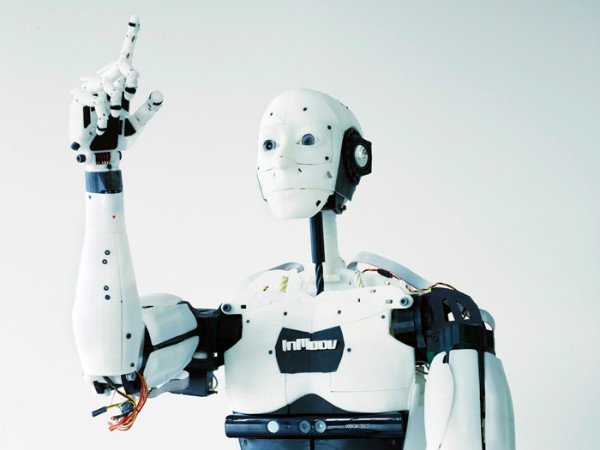
\includegraphics[scale=0.5]{images/Inmoov.jpg}
  \caption{The original form of the open source humanoid robot InMoov, which is designed by Gael Langevin. Image: Gael Langevin, from Wikipedia.}
  \label{fig:inmoov}
\end{figure}



The design framework was mainly influenced by two research papers which detail design frameworks for social robots \cite{bartneck2004design, huijnen2017implement}, with four articles defining design guidelines for robots used with autistic children acting as secondary influences \cite{designSpaces, giullian2010detailed, michaud2003characteristics, robins2007eliciting}.

\begin{figure}
\centering
  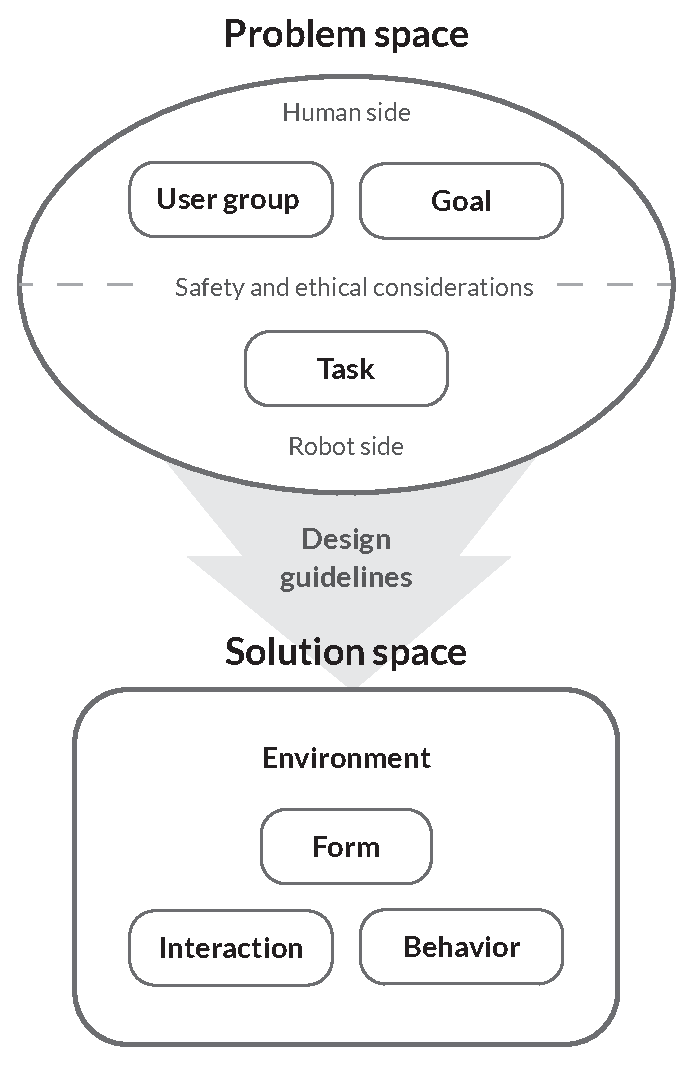
\includegraphics[scale=0.65]{images/designframework_v3.pdf}
  \caption{A proposed framework for the design of social robots. The design framework shows an abstraction of the process of design: first defining the problem space, then the design guidelines that emerge from that specific problem space, and the resulting solution space.}
  \label{fig:designframework}
\end{figure}

Huijnen implemented a co-creation design framework specifically for the design of robotic interventions for children with autism. The primary design dimensions which Huijnen describes are ``robot'', ``end-user'', ``environment'' and ``practical implementation'', which lead to a ``new intervention'' when defined \cite{huijnen2017implement}. Bartneck defined a design framework with five parameters: ``form'', ``modality'', ``social norms'', ``autonomy'' and ``interactivity''. Each parameter is rated along a scale, for example ``form'' ranges from abstract, to bimorphic, to anthropomoprhic \cite{bartneck2004design}. 

The structure of Huijnen's ``process'' was used to inspire the framework presented here. Huijnen first defined four dimensions, which led to the development of the new intervention \cite{huijnen2017implement}. Bartneck's idea of design parameters rated on ranges was incorporated into the design framework presented here \cite{bartneck2004design}. Additionally, four articles discussing the design requirements for robots to be used for autistic children specifically were examined for common design dimensions, although they were not explicitly mentioned in the articles \cite{designSpaces, giullian2010detailed, michaud2003characteristics, robins2007eliciting}.

The influence of these articles led to the realization of the process and design dimensions described in the framework presented here (figure \ref{fig:designframework}). First the design problem space is defined, which involves defining the user group, their goal, and the task of the robot. The problem space was examined already in the previous chapter: the nature of the user group and their issues and goals in therapy were discussed, along with the qualities of previous robots used in these interventions. The solution space is briefly discussed again in this chapter, as it is situated into the design framework. The qualities of the problem space lead to design guidelines, which were defined in the previous chapter. These design guidelines guide the decisions made in the solution space, which is discussed in this chapter. Defining the social robot as a solution involves making design decisions about its form, the way it can interact, and its behavior, which are all affected by the environment the robot is operating in.





\section{Relevant design theory}

The design framework is an abstraction of the design problems related to social robots, and decisions that need to be made when designing social robots in general. While in this thesis it is used for the specific purpose of designing a robot to teach assistive signs to children with autism, it can be used for the design of other social robots.

The design framework presented should be used at the start of the design process. It aids in defining the problem clearly for all individuals involved in the design process, as well as in considering all the dimensions relevant in the design process. The framework itself does not provide methods for granular design, but functions as a primer for considerations about the robot. When designing a robot with an interdisciplinary team, the design framework can be utilized as a boundary object, which helps bring knowledge into a material form, creating conditions for collaboration \cite{nicolini2012understanding}.

The framework describes the entire design process of a social robot, from problem space to solution space. The robot implemented here is used for a pilot study, so its design is a prototype, and is not planned to be the final version of the robot. Performing pilot studies with prototypes provides the opportunity to make ideas tangible faster, so that they can be evaluated and refined, and the best solution can be found faster \cite{brown2009change}. In use of the framework, after the implementation of the robot, another design iteration should be completed based on the examination of the initial implementation. This is a technique called iterative design, adapted from the design of computer user interfaces. Each iteration should be subjected to user testing or other usability evaluation \cite{nielsen1993iterative}. Iterations should be continued until the user issues have reached an acceptable level, or solved entirely. The iterative process to be used with the design framework for designing social robots is detailed in figure \ref{fig:designIterations}. In the case of this thesis, only one iteration was completed. User feedback is detailed in chapter \ref{chapter:results}, while what would be new design guidelines for the next iteration are discussed chapter \ref{chapter:discussion}.

\begin{figure}
\centering
  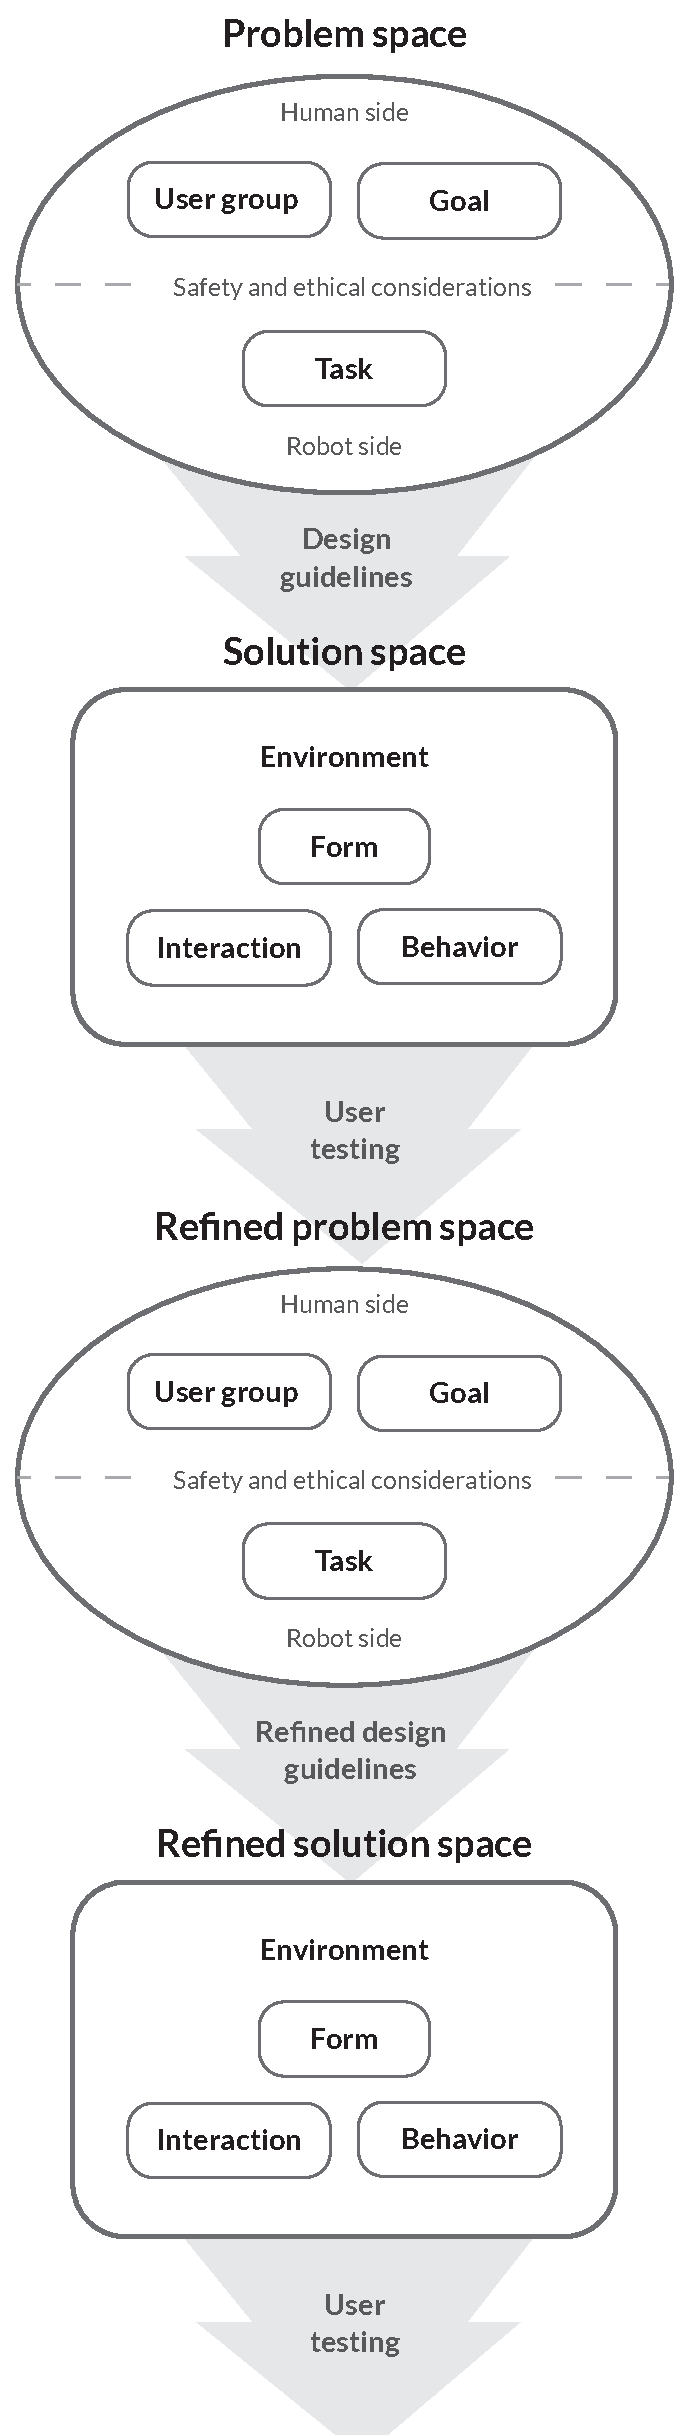
\includegraphics[scale=0.35]{images/design_iterations.pdf}
  \caption{The iterative design process to be utilized with the social robot design framework. After initial definition of the problem space, design guidelines and solution space, a round of user testing should take place. User testing evaluates the proposed solution, after which changes should be made. User testing could reveal that the original user group or their goal, the robot's task, or safety and ethical considerations were not adequately defined or constrained, which is why they should be re-examined after user testing. New design guidelines for the next iteration should be defined, and any existing design guidelines from the previous iteration that were not yet fully realized should be kept. The solution space should be refined and altered based on the user feedback.}
  \label{fig:designIterations}
\end{figure}


Designing social robots requires a deep understanding of human behavior and intelligence, in order to build their behavior in a way that seems intuitive to humans. Specifically, interdisciplinary knowledge and co-operation are needed, to build robots and applications that play a beneficial role in people's lives. Breazeal details a multidisciplinary approach where ``the design of social robot technologies and methodologies are informed by robotics, artificial intelligence, psychology, neuroscience, human factors, design, anthropology, and more.'' \cite{Breazeal2008}

As Breazeal recommends interdisciplinary collaboration, experts in the field of treating autism were consulted for the design of this robot. Designing the InMoov for use as an assistive sign teacher for autistic children involved two experts from the Satakunta hospital district, where the experiments would be performed. These experts were consulted during the definition of the dimensions of the robot in this design framework. Terhi Nyman is a psychologist specialized in neuropsychology, and the psychologist in-charge of social services at Satakunta's health care district. She has worked with people with autism and developmental disorders for over 10 years, and is well versed in the diagnosis and rehabilitation of ASDs and developmental disorders. Akuliina Lehtonen is a speech therapist who has been providing speech therapy for two years, and has over 10 years of experience of working with people with developmental and speech disorders. 

Knowledge of the experts was gathered during collaborative conversations where initial design decisions about the robot were made. Additionally, the speech therapist examined the robot and gave final suggestions before experiments were performed. Electronic communications were also utilized with both Lehtonen and Nyman to obtain additional knowledge. In this design process, new knowledge was created through the interaction between the tacit knowledge of the experts – which is converted into explicit knowledge through collaboration – and the explicit knowledge gathered from the theoretical research. This method of knowledge creation has been  described by Nonaka \cite{nonaka1995knowledge}. In the future, the knowledge of these experts should be captured by using the presented design framework as a boundary object of collaboration \cite{nicolini2012understanding}. By doing this, the experts will act more as participants in a co-design process, rather than external consultants. Experts should be involved in each design iteration. 


%%%%%%%%%%
%%%%%%%%%%
 
\section{Problem space}

Examining the problem space of designing a social robot involves defining the human side and the robot side of the problem (visible in figure \ref{fig:designframework}). Guiding the interaction between the two are safety and ethical considerations. These must be an integral part of any proposed solution, and so they must be discussed already during the definition of the problem.

\begin{figure}
\centering
  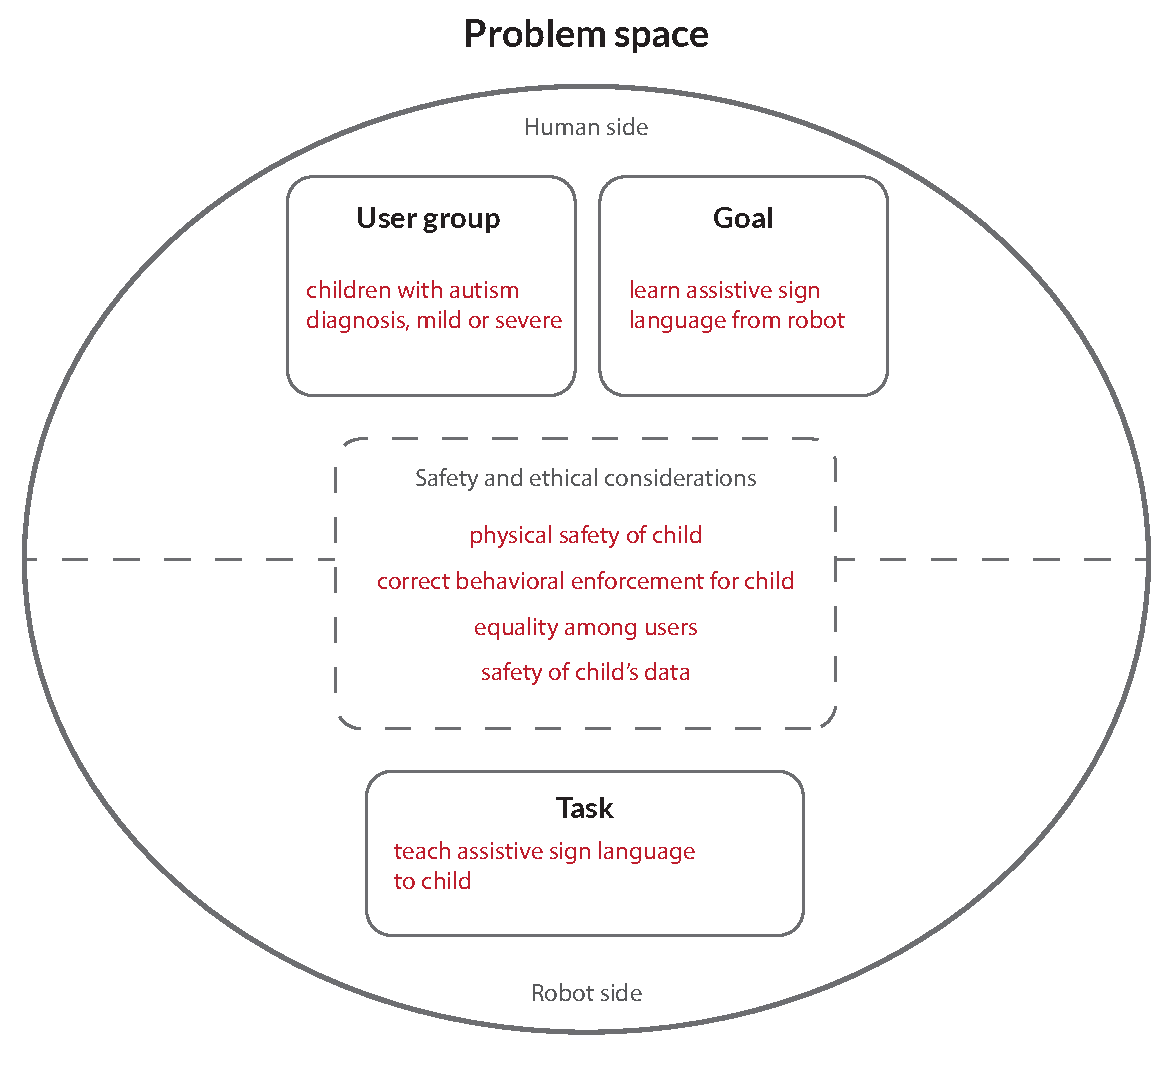
\includegraphics[scale=0.65]{images/problem_v1.pdf}
  \caption{The problem space of designing a social robot encompasses the user group, the user's goal, and the robot's task. Between the interactions of these two operators, safety and ethical considerations emerge.}
  \label{fig:problem}
\end{figure}




\subsection{User group}

On the human side, defining the user group is the first step toward defining the problem space. Defining a user group is important, in order to perform analysis on it and define what it needs. The user group is usually a specific demographic, with specific characteristics, whose needs and interests are steered by those characteristics. 

In this case, the user group is children with a diagnosis of either mild or severe autism (figure \ref{fig:problem}). The child should have the skill to recognize objects from photos, since this will be used with the robot as well. The child also should not have severe degradation of motor skills, so that they have the ability to learn signs. While children are different and have different preferences, some generalizations can be made based on the user group to design a starting point for the robot. 



\subsection{Goal}

After defining the user group, their goal is defined. A clearly defined goal helps examine the eventual solution's success, by whether it accomplished the defined goal for the user or not. The goal is specific to a user group, and should be thought of in terms of short-term and long-term goals.

In the case of autism therapy, therapeutic tools should have designs that have the goal of creating therapeutic value and meeting the individual, social and cognitive needs of the children involved in therapy \cite{designSpaces}. The goal for the users in this solution is to learn assistive signs from the robot (figure \ref{fig:problem}). The long-term goal would be for children to learn the signs on such a level that they are able to incorporate them into use in their daily lives. The short-term goal of the children is to successfully imitate the robot during the experiments. 


\subsection{Safety and ethical considerations}


Roboethics was a field established in 2004, which focuses on the human ethics of the robots' designers, manufacturers and users (instead of the robot and its artifical ethics). Roboethics are realized in the interaction between the robot and its user  \cite{Veruggio2008}. Safety and ethical considerations are important, as users may not always be aware of the potential negative consequences of using technology, and should be protected from negative effects by the designers of the robot.

In this design framework, safety and ethical considerations are realized on the border between the human side and the robot side (figure \ref{fig:designframework}). Safety and ethical considerations guide the definition of the problem space, and affect the design in the solution space. The safety and ethical treatment of both the user and their data should be taken into account. In this case, four considerations for the safety and ethical treatment of the user were defined for this robot-mediated intervention (figure \ref{fig:problem}). The implementation of these considerations is discussed in chapter \ref{chapter:solution}.

The physical safety of the child needs to be ensured while using the robot \cite{giullian2010detailed}. Machinery has the potential to crush or pinch the user if operated recklessly. 

Correct behavioral enforcement for the child was discussed with the psychologist and speech therapist. This means that the robot should not intend to replace human contact for the child, but to act as a tool to supplement learning. Mistreatment of the robot by the child should also be intervened in, so that the child learns that that behavior is not acceptable. Children have shown potential to treat social robots in an abusive manner when unsupervised \cite{brscic2015escaping}. Bad behavior toward social robots may even begin influencing children's behavior toward humans \cite{walk2016}. In this case, behavioral interventions were decided to be done by the human working with the child and the robot, rather than by the robot itself. Rewarding of the child when they behave correctly was also defined to be important for learning correct behavior.

Equality of the users was also discussed with the professionals. While the majority of children with autism diagnoses are boys, the number of female autism diagnoses has been steadily rising, faster than male diagnoses \cite{jensen2014time}. It has been argued that the lower number of female diagnoses is due to women being underdiagnosed with autism \cite{krahn2012extreme}. It has also been argued that males are generally more likely to be autists, as autism is a presentation of an ``extreme male brain'' \cite{baron2002extreme}. Due to disagreement on this matter, it was decided to keep the robot neutral in gender representation.

Data collected from experimental participants should be kept safely, especially in a medical context, in order to ensure privacy. Robots are in a unique data collection position when compared to personal computers, because they feel more social to humans, and elicit emotional responses \cite{calo2014case}, which may lead to the revelation of more personal data to the robot.  If data is used nefariously, especially sensitive emotional data that can be collected by a robot operating in a therapeutic context, there is potential for manipulation. It should be carefully considered what is an appropriate trade-off for users giving their data, and receiving a benefit from the processing of that data \cite{darling2015s}. In this case, the robot did not record any data, but data collected from the experiments was treated with the same respect.



\subsection{Task}

On the robot's side of the problem space, the robot's task is defined. The task is directly related to the user's goal. The task is the primary purpose for which the robot is built, and is what it needs to accomplish with the user. The build of the robot is completed once it can successfully accomplish the task. The task should also be thought of as both long-term and short-term.

In this case, the long-term task is teaching assistive sign language to the child. The short-term task is to produce the pre-defined signs accurately, and to respond to the child's behavior appropriately.


%%%%%%%%%%
%%%%%%%%%%


\section{Solution space}

\label{chapter:solution}

 \begin{figure}
 \centering
  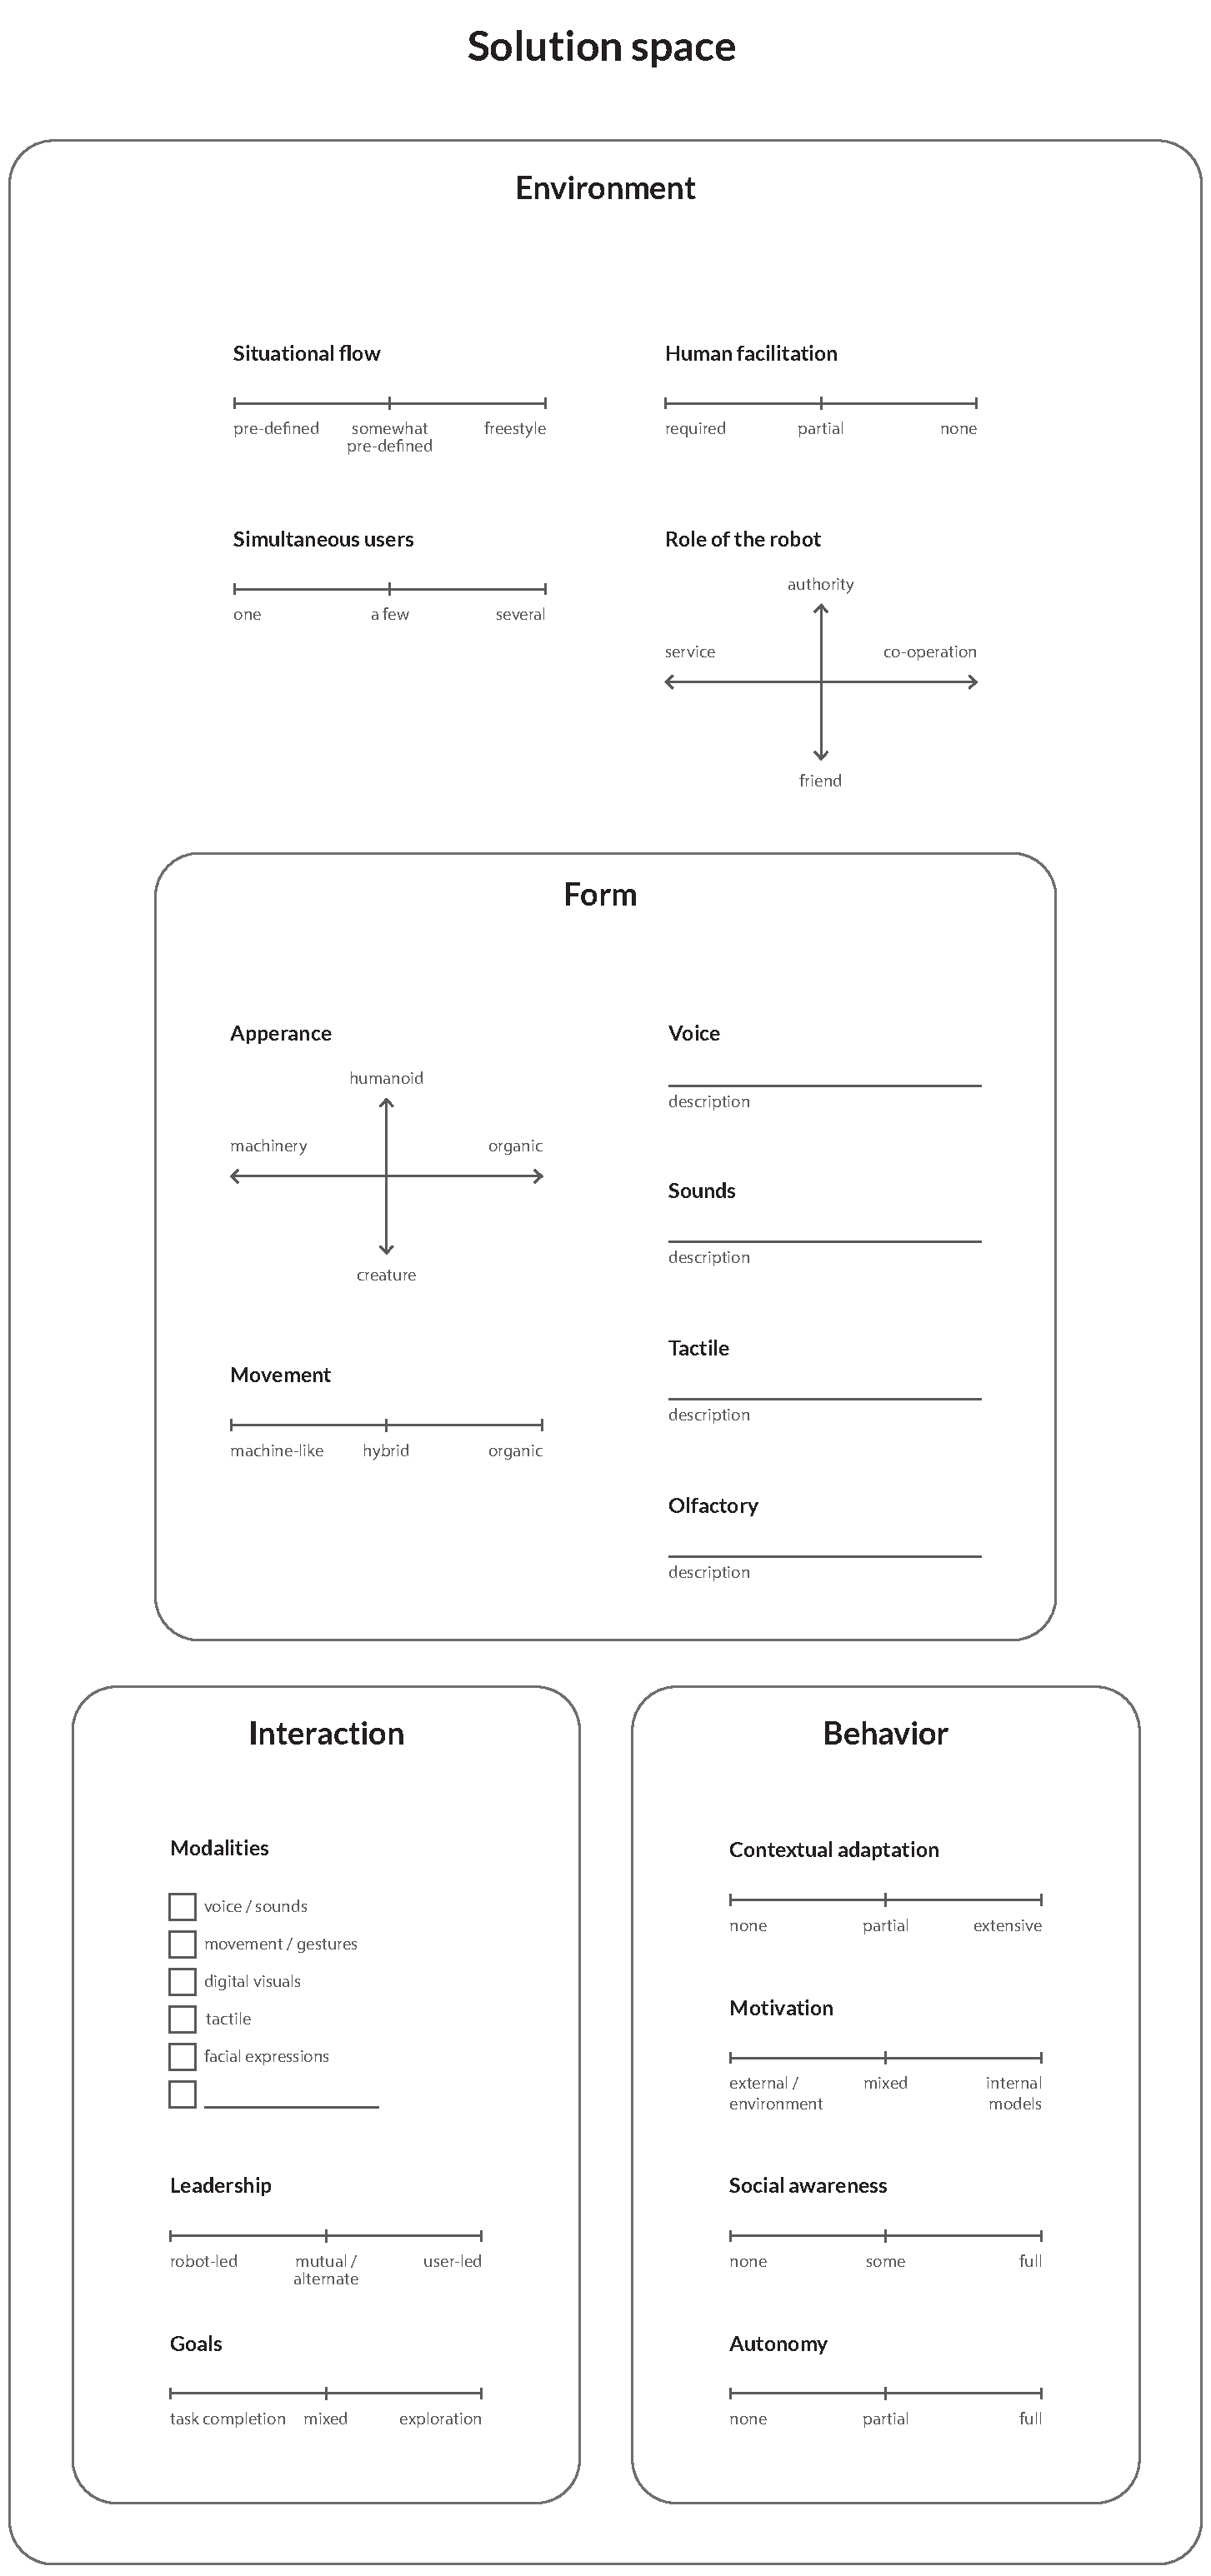
\includegraphics[scale=0.4]{images/solution_v4-01.pdf}
  \caption{Detailed depiction of the solution space in the framework for designing social robots. Defining the solution space involves designing the robot's environment, form, interaction and behaviors.}
  \label{fig:solution}
\end{figure}

The design of the solution space is guided by the design guidelines defined in the previous chapter, which were influenced by defining the problem space. Defining the solution space involves making decisions about the environment the robot operates in, which guides decisions made about its form, interaction and behavior (figure \ref{fig:solution}). In reality, these dimensions overlap each other, but this framework aims to make the interlinked decisions apparent and explicit.

The design guideline ``simple form'' specifically guides the form dimension, ``positive, supportive, rewarding experience and environment'' specifically guides the environment dimension, and ``consistent, structured, simple behavior'' specifically guides the behavior dimension. However, all these guidelines should be taken into consideration while designing other dimensions as well, as in reality the dimensions overlap each other. 

The guidelines ``modular complexity'' and ``modular specific to child's preferences'' can be realized in all dimensions. In this thesis, these two guidelines are specifically explored in the interaction dimension, and not touched on in the other dimensions. This is further explained in chapter \ref{chapter:interaction}. In a fully functional clinical solution, these two design guidelines should be realized in all dimensions.

In this case, the robot InMoov was chosen as the platform for the solution, due to availability. The selection of the InMoov creates some pre-defined constraints for the design of its form and interaction. Some of the pre-defined form and interaction qualities of the original InMoov are modified for this implementation. To modify the robot's form, its voice and sounds were modified from pre-set settings. To modify interaction qualities, new hands were added to give better signing ability, a tablet was attached to its chest, and lights were attached to one of its hands. These modifications are discussed in more detail below. Environment and behavior could be freely designed due to not being significantly limited by the InMoov.

First, the dimensions of the solution space are explained on a general level. Then, pre-defined constraints of the design defined by the InMoov are discussed. After this, the specific design for this solution, including modifications, is described. 


\subsection{Environment}

\label{chapter:environment}
\label{sec:environments}

In this framework the environment does not mean the location of the robot, but rather all factors surrounding its operation. The environment is examined through four qualities: situational flow, simultaneous users, human facilitation and role of the robot, as seen in figure \ref{fig:environment}. The design driver ``positive, supportive, rewarding experience and environment'' guides the design of this dimension. 


 \begin{figure}
  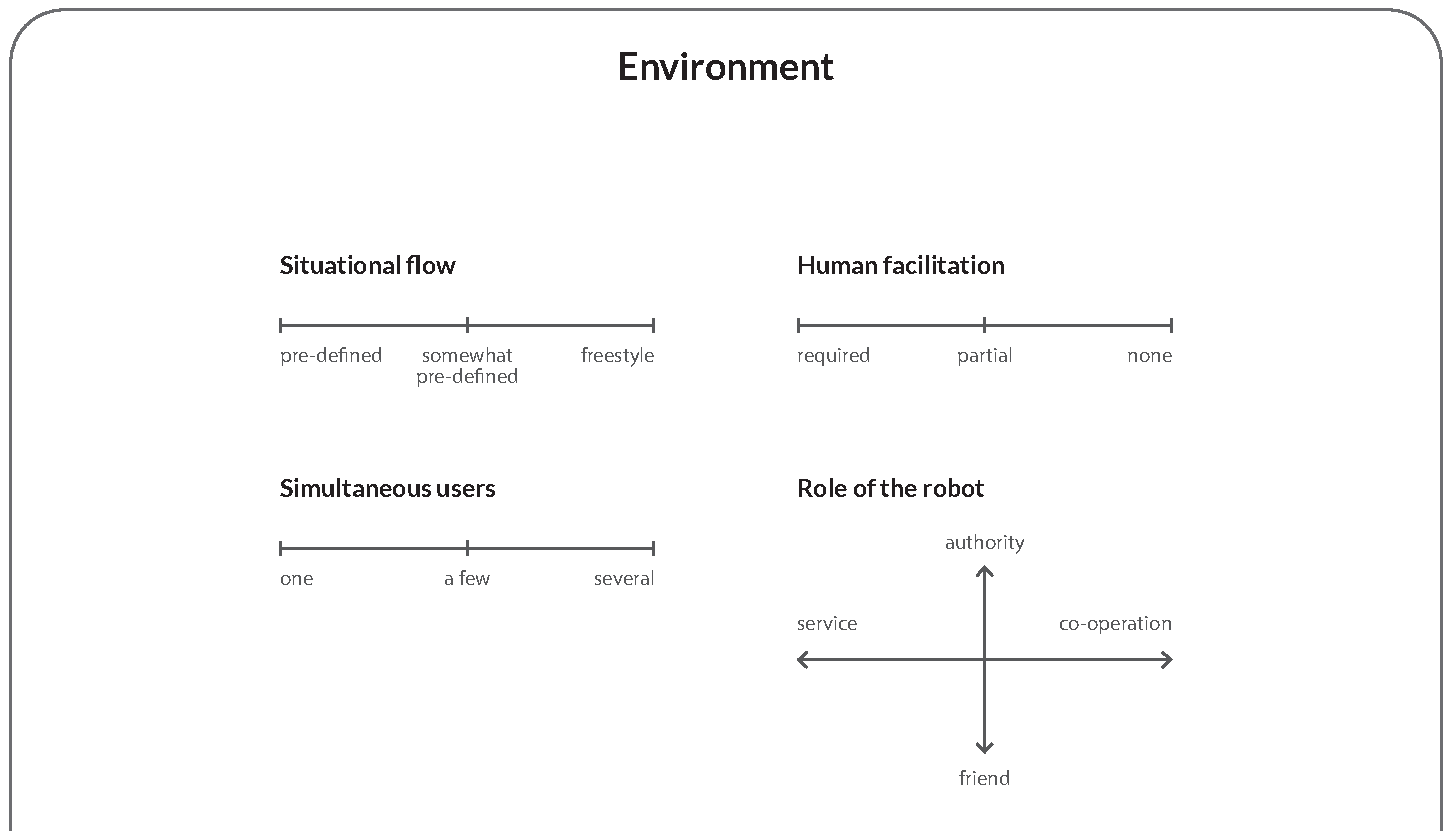
\includegraphics[width=\linewidth]{images/solution_v4-02.pdf}
  \caption{Defining the environment of the social robot involves examining the nature of the situational flow of the interaction with the robot, and the step preceding and following it. It also involves making decisions about the number of simultaneous users, the level of human facilitation needed in the solution, and the nature of the role of the robot in its environment. The environment affects design decisions made of the robot's form, interactions and behavior.}
  \label{fig:environment}
\end{figure}

The design choices made for the environment of the solution in this case can be seen in figure \ref{fig:environmentFinal}.


\begin{figure}
  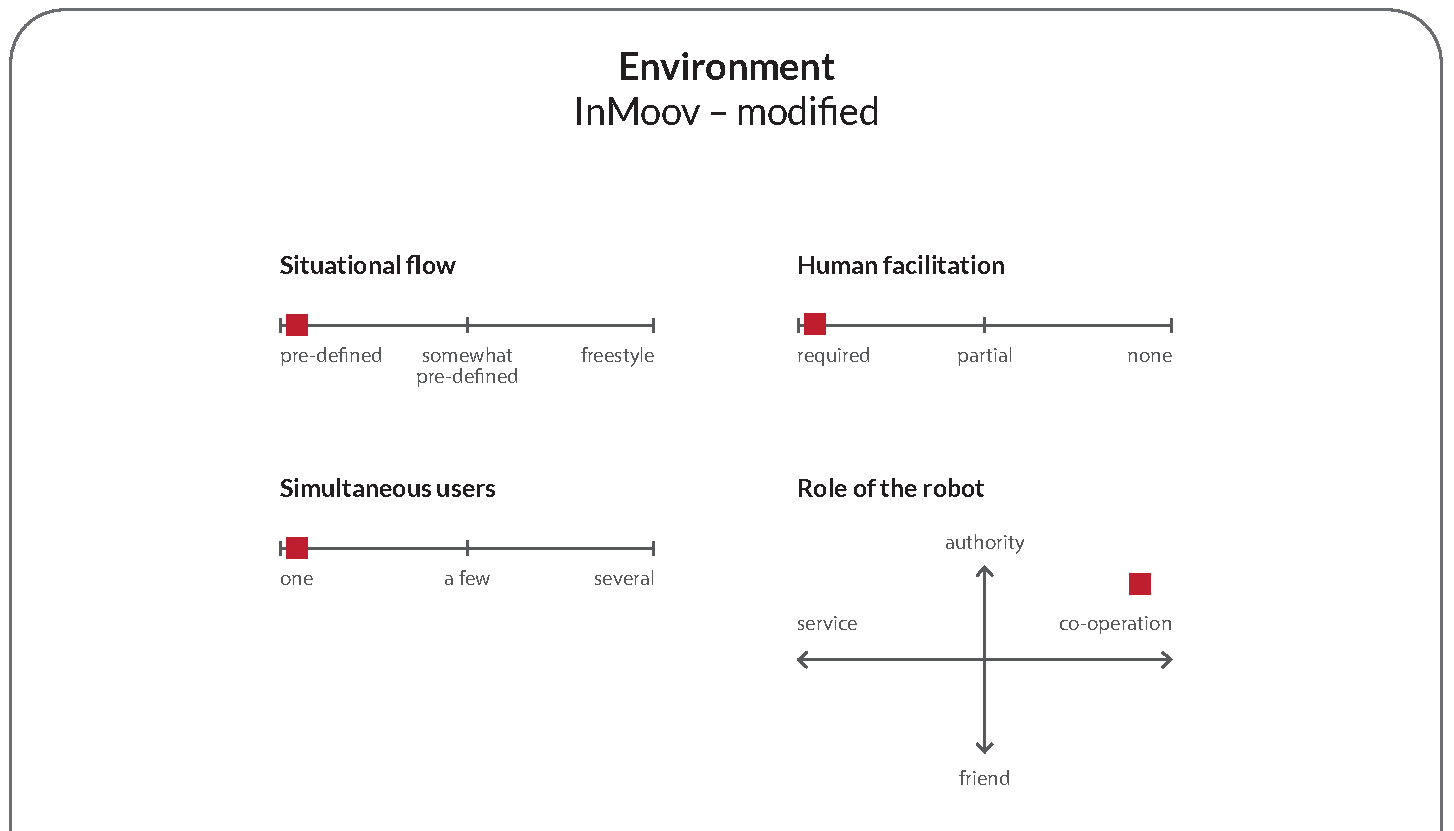
\includegraphics[width=\linewidth]{images/solution_inmoov_final-02.pdf}
  \caption{Design choices made about the environment of the solution provided with the InMoov, shown in red.}
  \label{fig:environmentFinal}
\end{figure}


\subsubsection{Situational flow}

The situational flow describes how pre-defined the environment surrounding the interaction with the robot are, ranging from pre-defined, to somewhat defined, to freestyle. Situational flow describes how exactly the events leading up to and after the interaction with the robot are defined.

The situational flow of this solution is highly pre-defined, as seen in figure \ref{fig:environmentFinal}. What happens before and after the therapy situation is rigidly pre-defined, since people with autism prefer routine and unexpected situations may upset them \cite{frith2003autism, tetzchner}. The child is accompanied by their companion and the speech therapist when going into and out of the room, in order to support them during what may be a stressful experience. The exact experimental procedure is detailed in chapter \ref{chapter:methods}. This follows the ``positive, supportive, rewarding experience and environment'' design guideline.


\subsubsection{Simultaneous users}

Simultaneous users describes how many users interact with the robot simultaneously in the environment.

In this case, there is only one user, due to the pilot nature of the study. This thesis aims to observe the direct interaction between one child and the robot. In future interventions, children could potentially interact with the robot and another child, or another person. This would require re-designing the environment of the robot accordingly.


\subsubsection{Human facilitation}

The level of human facilitation of the environment describes whether the interaction between the robot and the user needs another human's support to move forward. If the robot is part of a chain of events in which humans are involved, human facilitation is required. If the robot freely exists in a space, with users free to interact with it as they please, there is no human facilitation. Partial human facilitation can for example mean a designated human guiding users toward the robot.

The use of a robot in this context needs human facilitation. The child should not be alone with the robot due to safety and ethical concerns discussed in the problem space: physical safety of the child and correct behavior reinforcement. To ensure the physical safety of the child, the robot has a quickly activated stop button in case of emergencies, as recommended \cite{giullian2010detailed}. However, intervention by a human facilitator is the primary way of preventing the child from getting too close to the robot and injuring themselves. The presence of another human also ensures correct behavioral reinforcement, by ensuring that the robot does not replace human contact, and by intervening if the child were to mistreat the robot. 

The operation of the robot from the control room is made easier with a human facilitator. The human facilitator, in this case the speech therapist, signals to the operator how the robot should behave. A companion of the child, meaning a parent or other caretaker, is also present in the therapy to help the child feel safe and calm. This follows the ``positive, supportive, rewarding experience and environment'' design guideline.


\subsubsection{Role of the robot}

The role of a robot is highly variable. Huijnen defines the roles of robots used in autism therapy as ``provoker'', ``reinforcer'', ``trainer'', ``mediator'', ``prompter'', ``diagnoser'', and ``buddy'' \cite{huijnen2017implement}. However, for the general design of social robots, these roles are too few. Because all possible roles can not be listed in a design framework, a two-dimensional map is implemented, within which roles can be situated. There are two ranges, from service to co-operation, and authority to friend. This describes the robot's relationship to the user in the given environment. The robot can either serve the user, or they can co-operate on a task. The robot can act as an authority with the user, maintaining distance, or it can act as a friend, feeling closer to the user. The robot does not have to be strictly one or the other, but can fall into sub-divisions on the map.

In this solution, the robot is an authority for the child. Becoming more of a friend would require physical contact (as with for example Probo, the huggable robot \cite{ProboRef}), which was not possible due to the fragility of the InMoov. The robot being framed as an authority can also help the child focus on the task at hand and follow its instructions, and not on ``making friends'' with the robot. 

The robot is more of a co-operator than a server. The robot and the child take turns signing, thus working together, rather than the robot performing a task for the child.

To create a supportive and rewarding experience as a co-operating authority, the robot should reward the child when they sign correctly. If the child signs incorrectly or does not react, however, the robot is not critical, and is supportive of the child. This follows the ``positive, supportive, rewarding experience and environment'' design guideline.


\subsection{Form}

\label{chapter:form}

The form of the robot encompasses all its externally perceptible qualities. Defining the form of the robot involves examining six qualities: appearance, movement, voice, sounds, tactile sensations and olfactory sensations, as seen in figure \ref{fig:form}. ``Simple form'' is the primary design guideline of this solution dimension.

\begin{figure}
  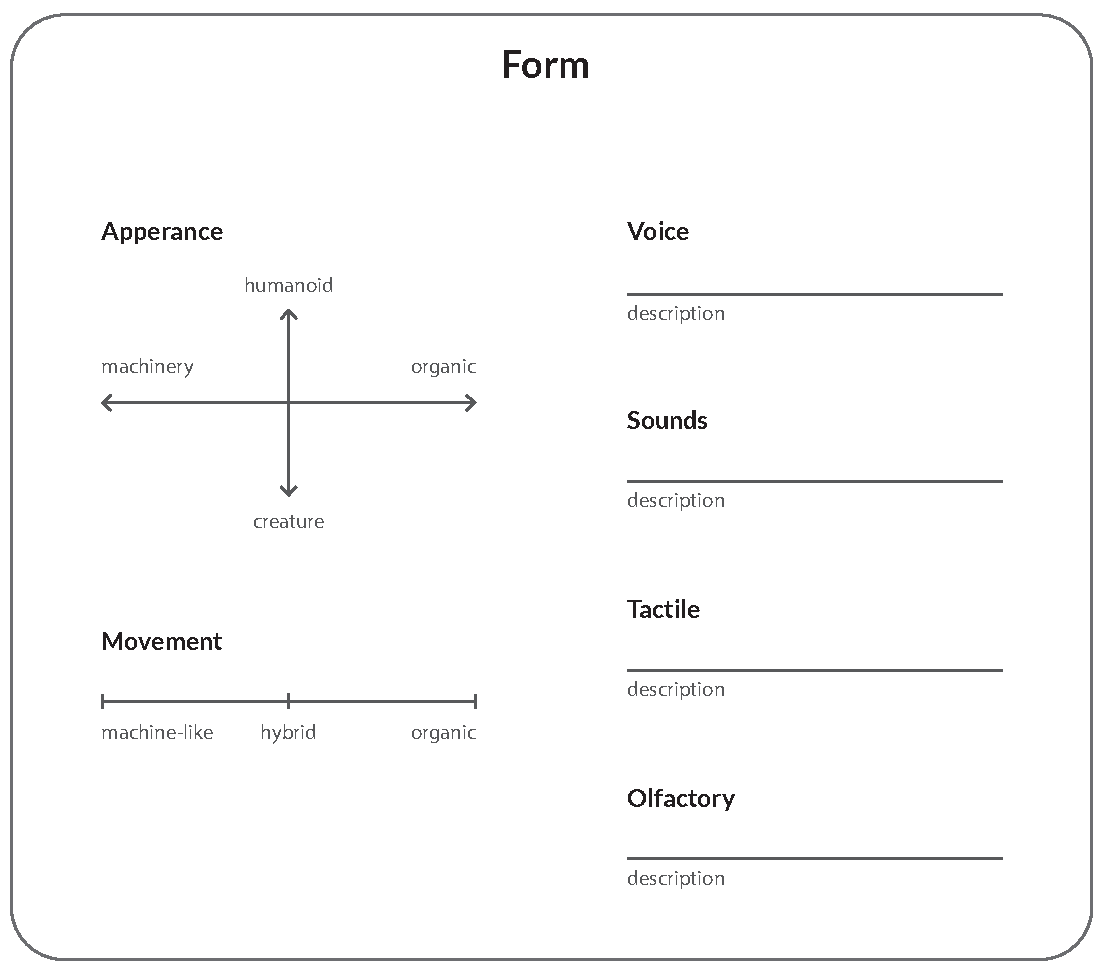
\includegraphics[width=\linewidth]{images/solution_v4-03.pdf}
  \caption{Defining the form of a social robot involves making decisions about its appearance, the way it moves, its voice and sounds, and tactile and olfactory sensations. As voice, sounds, tactile and olfactory sensations are all highly variable, freeform descriptions are used.}
  \label{fig:form}
\end{figure}

A well-known measure of a robot's form in the field of robotics is evaluating the robot according to its ``familiarity'' to life. This is defined by the degree to which the robot resembles human-like appearance and movements. It is argued that a robot should not be too human-like, or it will fall into the ``uncanny valley" of negative familiarity, appearing like an animated corpse. The original theory of the ``uncanny valley" suggests that a robot should not be made to be too human-like, as a safe familiarity can be produced by a design approaching human likeness, but not too close to it \cite{mori1970uncanny}. This theory can be further expanded into creature-like robots: they should not be made too life-like, to avoid appearing zombie-like. The appropriate degree of familiarity according to this theory is generally accepted in the field of robotics, which is why it is not introduced as a variable in this framework. This accepted level of familiarity – approaching human or creature likeness, but not attempting to be an exact copy – can be achieved by appropriately designing the qualities that make up the robot's form. All dimensions of the robot's form contribute toward its life-likeness, with appearance and movement being most important.

In this case, defining the form of the robot for the solution had some constraints, due to selection of the InMoov as a solution platform. Pre-defined form qualities are visible in figure \ref{fig:formPredefined}. The original form of the InMoov (figure \ref{fig:inmoov}) is used as a base, and modified according to the established design guidelines, and safety and ethical considerations. The modifications done to the InMoov's form can be seen in figure \ref{fig:formFinal}. The open source nature of the InMoov makes modifying it possible. Modifying the robot's voice and sounds is possible through its open source MyRobotLab software.


\begin{figure}[htbp]
  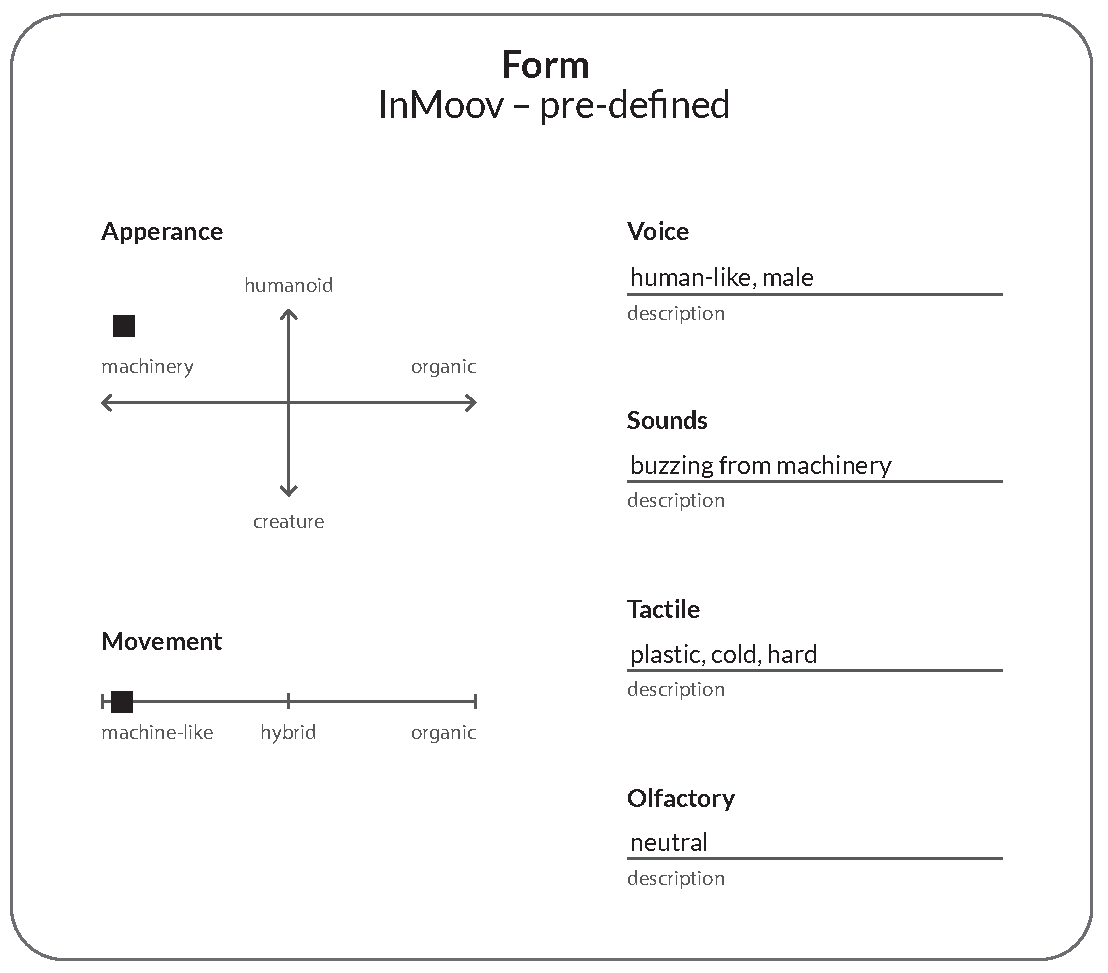
\includegraphics[width=\linewidth]{images/solution_inmoov_predefined-02.pdf}
  \caption{The choice of InMoov as the solution platform set the baseline for form design.}
  \label{fig:formPredefined}
\end{figure}


\begin{figure}
  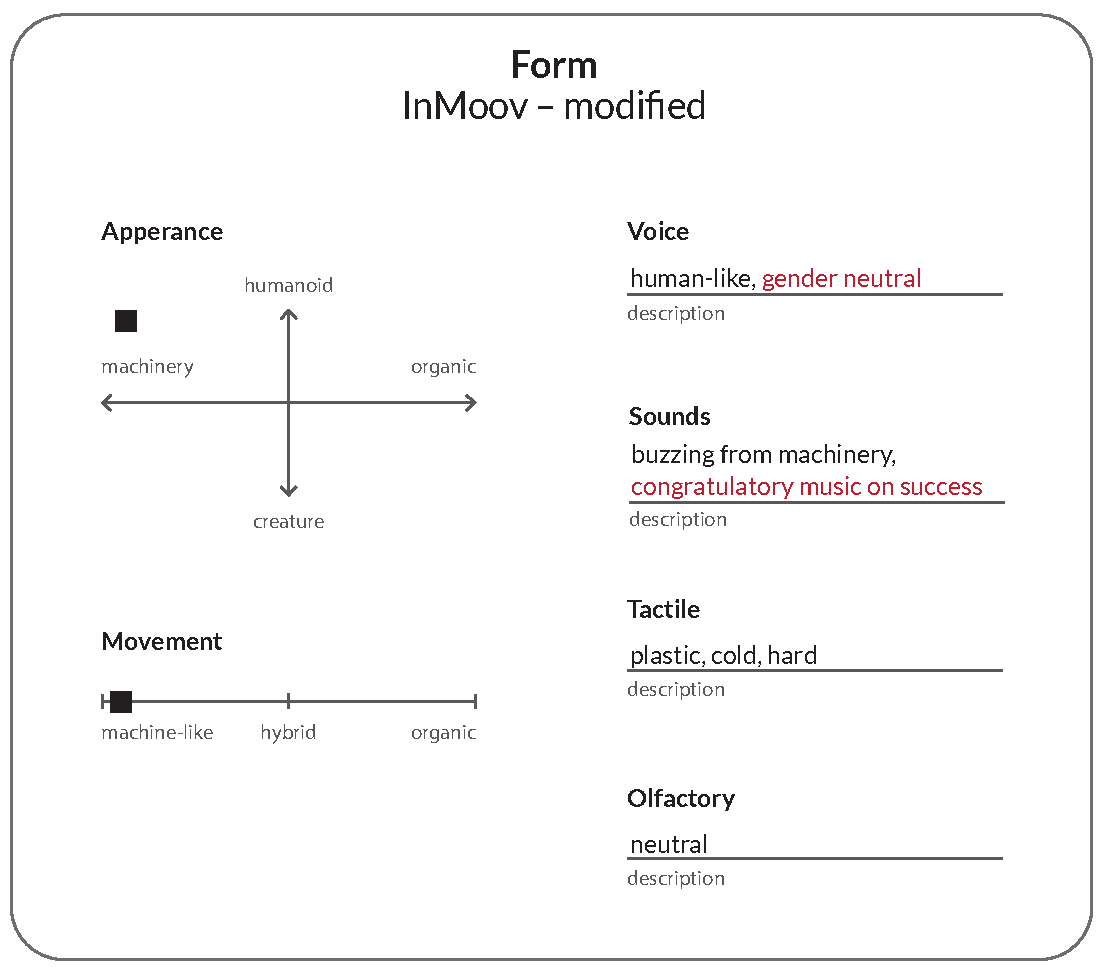
\includegraphics[width=\linewidth]{images/solution_inmoov_final-03.pdf}
  \caption{The design baseline of the form pre-defined by the InMoov is shown in black, and the modifications made to it are shown in red.}
  \label{fig:formFinal}
\end{figure}


\subsubsection{Appearance}


The appearance of a robot is highly variable, which is why a two-dimensional map is used to describe it. In this framework, the appearance can range from machine-like to organic, and from humanoid to creature-like. The appearance of a robot defines the user's initial response to it. If a robot appears sophisticated, the user will assume similar level of sophistication in its skills \cite{bartneck2004design,designSpaces}. A humanoid robot is perceived as human-like, and elicits strong expectations about the robot's social and cognitive competencies \cite{designSpaces}, while a creature-like robot is perceived as more of an animal, with a lower level of functioning. 

The appearance of the robot was not modified significantly from the base InMoov design. The only modifications to the robot's appearance were done for the sake of interaction, and are discussed in chapter \ref{chapter:interaction}. The humanoid design of the InMoov is suitable for this solution, as the goal is for autistic children to use the humanoid robot to practice skills related to human-to-human communication \cite{designSpaces}. The robot is mechanical in appearance, but not so mechanical that the child would be more interested in examining its components, rather than interacting with it. The robot is easily discernible as humanoid, but also robotic enough to not be confused with a human \cite{giullian2010detailed}.

The InMoov's original face design was also suitable for this solution. The face is simple with distinct features, with no ability for facial expressions. Complex affective expression by human faces have been shown to cause an overstimulation effect in autistic people's brains, which in turn leads to gaze avoidance by the autistic person \cite{dalton2005gaze}. A simple face helps prevent overstimulation, confusion and avoidance \cite{giullian2010detailed}.

The robot was not modified to appear more human, which could have been done with clothing or a wig. This was decided in agreement with the speech therapist and psychologist. This also follows the design guideline of ``simple form''.


\subsubsection{Movement}

In this framework, the movement of a robot can be rated from machine-like, to hybrid, to organic. Organic, smooth movements suggest a more sophisticated robot in terms of skills, while a more mechanical movement quality suggests a more rudimental robot.

It has also been argued that robotic movements, in contrast to human movements, elicit a faster imitation response from autistic children \cite{pierno2008robotic}. However, in this case, the speech therapist recommended that the robot have movements that are as smooth as possible, in order to sign as accurately as possible. The InMoov's base level of movement is machine-like, and difficult to modify. In order to take into account the speech therapist's advice, the InMoov's original hands were replaced with different hands, in order to give the fingers and wrists smoother movements. The robot does not over-extend its limbs, and does not assume positions impossible for humans \cite{giullian2010detailed}.


\subsubsection{Voice and sound}

The robot's voice and the sounds it makes contribute to the robot's life-likeness. A voice can be robotic, or human-like. Voice can be perceived to have a gender or an age, which depends on speed, pitch and other qualities. Voices, both robotic and human-like, can have tonality, being either monotone or having vibrant prosody. The noises a robot can make are almost infinitely variable: machine-like ``beeps", music, human-like exclamations or animal calls are common examples of sounds a robot can make. The sounds that a robot's machinery may make when it moves are also part of its soundscape. A robot's soundscape can also include sounds that it makes when it is touched, or if it is mobile, sounds that it makes when it moves in space.

In this framework, voice and sounds are defined through a free-form description, as they are both highly variable. Measurements via ranges or maps, as are done for the appearance and movement, could be developed in the future, in collaboration with an expert in audio.


The original voice of the InMoov was a human-like male, as seen in figure \ref{fig:formPredefined}. It was decided that the robot should keep a human-like voice, in order to make it more natural to practice human-to-human interaction with. Due to the decision to keep the robot gender-neutral, which was discussed in the definition of the problem space, its voice was modified. A female Finnish-speaking human-like voice, Satu from Apple, was used. Its pitch was lowered to make it indistinguishable as either a male or female voice. Prosody of the voice is defined by the Satu system, which mimics human-like tonality. The voice of the robot was also slowed by 10 \% from the original Satu voice, to make it more understandable to the children.

The robot plays a short congratulatory musical tune through its mouth speaker when a child signs successfully. This provides a sensory reward for the child \cite{robins2007eliciting, michaud2003characteristics}, which follows the design guideline of ``positive, supportive, rewarding experience and environment". 

The InMoov's machinery is quite noisy, and gives off a buzzing sound as it moves its hands. The InMoov's material does not give off sound when touched. The InMoov as a whole is fixed in place, and thus there are no sounds resulting from the robot moving from point to point.


\subsubsection{Tactile sensations}

Tactile sensations are especially important if the user is in close contact with the robot. Soft and warm tactile sensations suggest comfort and familiarity, while hard and cold tactile sensations suggest distance and industrial qualities.

In this framework, free-form descriptions are used to describe tactile sensations, as they are highly variable. In the future, measurements such as ranges or maps could be developed to describe these qualities.

In this solution, tactile properties were pre-defined by the choice of using InMoov as a solution platform. The material used to construct the InMoov is a cold, hard plastic, which suggests distance. However, as the planned interactions with the robot do not include touching it, tactile sensations do not need to be taken into account or modified.


\subsubsection{Olfactory sensations}

Olfactory sensations are also especially important if the user is in close contact with the robot. Olfactory sensations can induce sensations of pleasure or disgust, or they can be entirely neutral.

In this framework, olfactory sensations are defined through a free-form description, as they are highly variable. In the future, ranges or maps could be developed to describe these sensations. 

The olfactory sensations are pre-defined by the InMoov's material, as plastic has no smell and is thus neutral. In this case, there was no need to modify the sensations, as users would not be in close contact with the robot, and could not smell it. 


\subsection{Interaction}

\label{chapter:interaction}

The interaction dimension defines the manner in which a user can interact with a robot. In this framework, interaction is examined through three qualities: modalities, leadership, and goals (figure \ref{fig:interaction}). 

\begin{figure}
\centering
  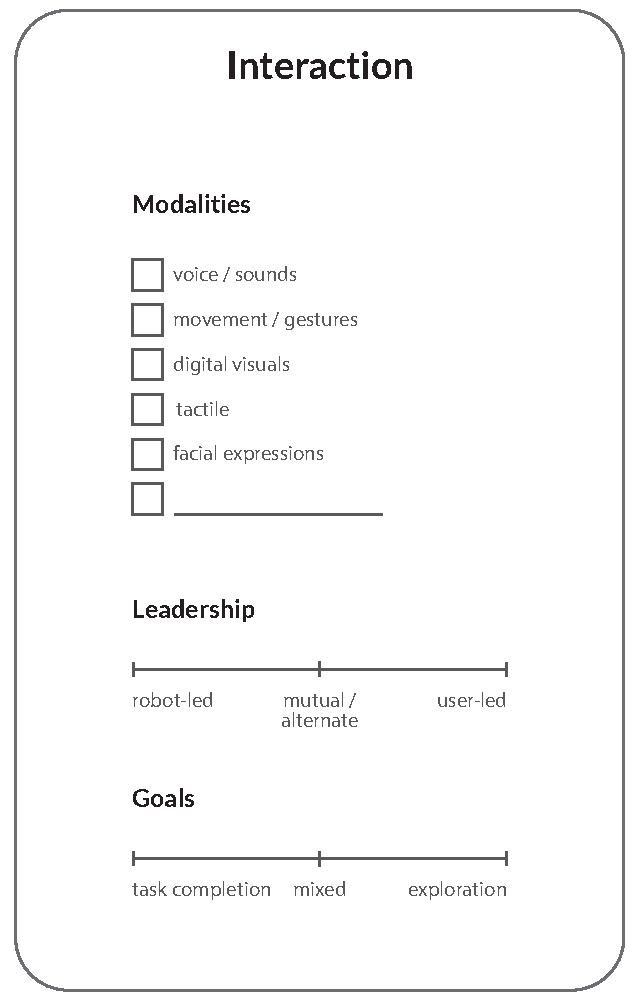
\includegraphics[scale=0.75]{images/solution_v4-04.pdf}
  \caption{The interaction design dimension contains interaction modalities, which can be expanded upon from the list available, leadership of the interactions, and the robot's goals in performing the interactions.}
  \label{fig:interaction}
\end{figure}

No design guidelines defined in the previous chapter specifically guide the interaction dimension. However, the design guidelines ``modular complexity" and ``modular specific to child's preferences" can both be realized in the design of interactions. 

In this thesis, different modalities of interaction are compared. These modalities are used to examine modularity of the robot. In the future, modular qualities of the robot can be used to fulfill the design guidelines of ``modular complexity" and ``modular specific to child's preferences". Due to the pilot nature of this study, these design guidelines are not yet fully realized.

Due to the overlapping nature of the design dimensions, interaction is somewhat pre-defined by the form of the robot. Interacting with the InMoov involves the modalities of voice and gestures, due to the design of the robot's form. The pre-defined interaction qualities are visible in figure \ref{fig:interactionPredefined}, and modifications made to the interaction dimension are seen in figure \ref{fig:interactionFinal}.


\begin{figure}
\centering
  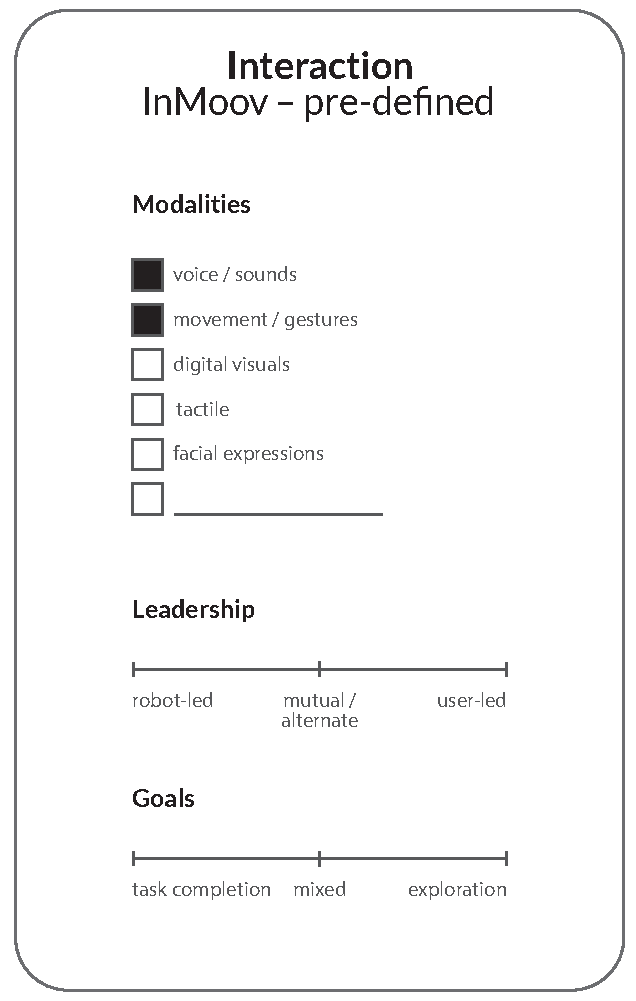
\includegraphics[scale=0.75]{images/solution_inmoov_predefined-03.pdf}
  \caption{InMoov has the pre-set interactions modalities of voice and sounds, and movement and gestures, which set the baseline for design.}
  \label{fig:interactionPredefined}
\end{figure}

\begin{figure}
\centering
  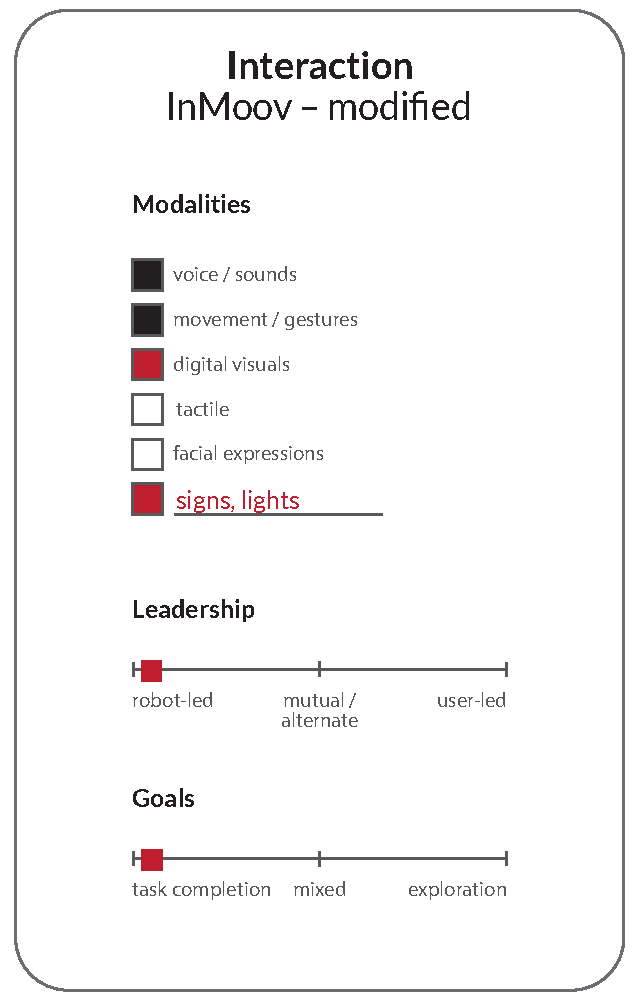
\includegraphics[scale=0.75]{images/solution_inmoov_final-04.pdf}
  \caption{The design baseline for interactions pre-defined by the InMoov are shown in black, and the additions made to it are shown in red.}
  \label{fig:interactionFinal}
\end{figure}



\subsubsection{Modalities}

Modalities of interaction define the different ways a user can interact and communicate with the robot. Modalities of interaction can vary greatly. A list of the most common modalities encountered in interaction with robots are listed in this framework. Additionally, an empty space for novel modalities is provided. Modalities are restricted by what human senses can perceive. Even though a robot could theoretically communicate via radio frequency, a human can not do this, so interaction through this modality is not possible. Robots can interact via multiple modalities, either simultaneously or one after the other.

For this solution, interaction modalities were discussed with the psychologist and speech therapist, and determined to be a special area of interest in communication therapy with a robot. Increasing the complexity of a communication prompt according to the child's skills has been studied previously \cite{ARIA, pop2013social}. This could be done by using modalities that are more complex in quality, or combining different modalities with each other to produce a more complex prompt. 

Here, three different interaction schemes – constructed out of different interaction modalities – are compared with each other. The schemes could potentially be used to increase complexity, or selected specifically to suit a child's preferences. However, in this solution, the schemes are not chosen specific to complexity or child. The schemes are examined in isolation, in order to separate the effect of each scheme. The specific organization of the interaction schemes during the interaction is further examined in chapter \ref{chapter:methods}. The schemes can be thought of as three separate design conditions.

Interaction modalities used in this solution are voice and sounds, gestures, digital visuals, lights and signs. Voice and sounds were discussed in chapter \ref{chapter:form}.

Visual elements such as photos can be used to aid communication with autistic individuals \cite{tetzchner, michaud2003characteristics}. One of the interaction modalities chosen was to display digital visuals from a tablet planted into the robots chest, as inspired by Probo \cite{pop2013social}. This way, the InMoov could show an image of the word being signed. The robot's open source nature made this possible, as the new parts that were needed for the chest could be easily designed and 3D printed.

Lights can be used to capture the interest of autistic children \cite{michaud2003characteristics}. Lights have been observed to be a good attention grabbing and maintaining tool in an experiment where autistic children played turn-taking games with colorful light-up blocks \cite{brok2010engaging}. Small LED lights were attached to the robot's hand, which flash when it signs. 

Signing is a novel interaction modality. Better signing was accomplished due to the new hands attached to the robot. To keep from confusing the child, movement is otherwise kept to a minimum. In addition to the signs, the robot uses only three communicative gestures: waving hello when the child arrives, waving goodbye when the child leaves, and showing a thumbs up when they succeed in signing correctly. No other body language, such as using gaze direction or body orientation to direct attention is used.


\subsubsection{Leadership}

The leadership of the interaction describes who drives the interaction forward, and takes initiative. Leadership can range from robot-led, to mutual or alternate, to user-led. Leadership defines whether the user feels that they are controlling the robot's actions, or if the robot is guiding the user to act a certain way.

In this solution, the interactions are initiated and led by the robot. During the interactions, the robot signs, and asks the child to imitate. The robot explains the rules of the game to the child when they enter the room. The robot always signs first and then asks the child to imitate the sign. The robot also ends the interaction with a goodbye. 


\subsubsection{Goals}

The goals of the interaction relate back to the goal of the user defined in the problem space (figure \ref{fig:problem}). The interaction can have only one, or multiple goals. The goal of the interaction for the user can be to complete a task, or exploratory in nature. When the goal is to complete a task, it is clear when the task has been accomplished. An exploratory interaction can for example generate knowledge, pleasure, or a novel experience for the user. The goal or goals of interacting can also be a mix of exploration and task completion.

For the InMoov, the goal of the interaction is task completion. The robot's goal is to successfully teach the child assistive signs through imitation.



\subsection{Behavior}

\begin{figure}
\centering
  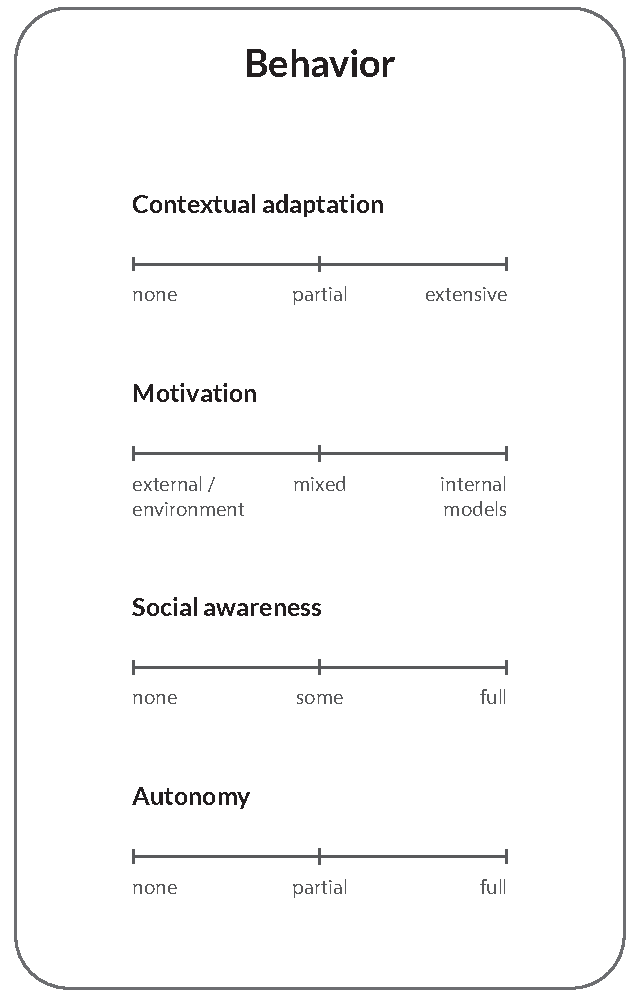
\includegraphics[scale=0.75]{images/solution_v4-05.pdf}
  \caption{Behavior design involves defining the level of contextual adaptation of the robots behavior, the motivation for behaviors, the level of social awareness evidenced in behavior, and the level of autonomous behaving of the robot.}
  \label{fig:behavior}
\end{figure}

The behavior dimension defines how the robot acts. Behavioral design is important, as the robot's behavior is one of the primary determinants of the user's attitude toward it, and contributes to its life-like impression \cite{designSpaces}. Behavior is defined by four qualities: contextual adaptation, motivation, social awareness and autonomy (as seen in figure \ref{fig:behavior}). ``Consistent, structured, simple behavior" guides the design of the behavior dimension. The design decisions made about the InMoov's behavior are seen in figure \ref{fig:behaviorFinal}.



\begin{figure}
\centering
  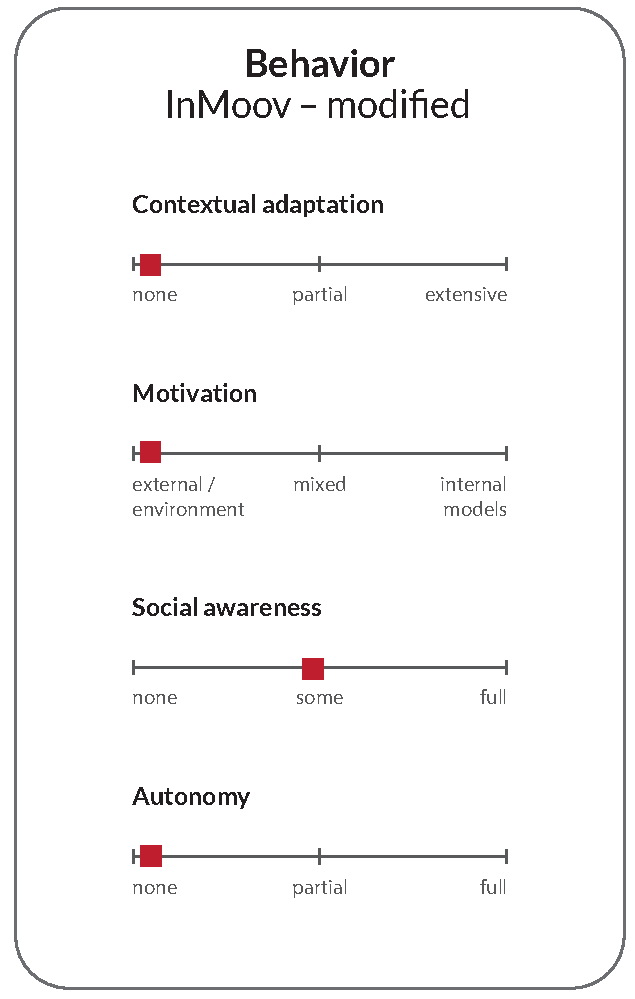
\includegraphics[scale=0.75]{images/solution_inmoov_final-05.pdf}
  \caption{The design decisions made about the InMoov's behavior in this solution are showed in red.}
  \label{fig:behaviorFinal}
\end{figure}


\subsubsection{Contextual adaptation}

Contextual adaptation of behavior refers to how much of the robot's behavior has been defined beforehand by its creator, and how much the robot can independently determine its behavior according to the context. The levels of contextual adaptation of a robot's behaviour range from none, to partial, to extensive. Extensive adaptation is a description of human-like behavior, where the agent could improvise and adapt to different contexts and domains. Currently, to my knowledge, no robots exist that could perform a similar level of adaptation to humans. Behavior that can be classified as extensive contextual adaptation would involve the robot taking input from past situations that it has learned from, as well as the current context, and determining the best course of action according to these. If a robot were to perform on a similar level as a human, it would need to be able to learn to improve its decision making process and behavior according to success of past tasks. Robots that exhibit no contextual adaptation always follow the same course of action in a given situation. Their behavior is ``hard-coded".

At the time of writing, robots generally exhibit no contextual adaptation, or partial contextual adaptation. An example of partial contextual adaptation could be a robot behaving in a particular way in a given situation, but with randomized adaptations. By performing randomized behavior, a robot can modify its future behavior based on the best outcomes, and become more efficient in partial adaptation. For example, "artist robots" can create artwork by randomizing certain artistic styles onto pre-determined images. The choice of artistic style is based on data from previous sales of paintings, which leads to the robot attempting to improve its performance with each iteration. Here, while the robot appears to be behaving in a creative and improvisational manner, it does not take into consideration the context of the image being created. It also could not apply its artistic skills in another context. This leads to the behavior being classified as having partial contextual adaptation.

The behavior of the InMoov has no contextual adaptation. The signs and speech of the robot need to be pre-programmed. Hard coded behavior is also more consistent and structured than adaptation, which leads to less confusion for the child. Children can learn to imitate the robot more easily, due to the repetitiveness of the robot's imitation prompts. This follows the design guideline of ``consistent, structured, simple behavior". 


\subsubsection{Motivation}

Motivation of behavior describes whether the robot behaves purely in response to external stimulus from its environment, purely according to internal models, or a mix of the two. An example of motivation via internal models is the motivation system of the robot Kismet, in which behaviors are influenced according to internal models of Kismet's drives and emotions \cite{breazeal2004}.

In this solution, everything the robot does in the therapy situation is motivated by what the child is doing, which means that motivation is entirely external. The robot has no programmed ``internal models". Keeping the robot's behavior externally motivated follows the design guideline of ``consistent, structured, simple behavior", since children with autism have trouble anticipating other's internally motivated behavior due to lack of Theory of Mind \cite{baron1985does, frith2003autism}.



\subsubsection{Social awareness}

Designing social behavior to the right degree is difficult, as a robot may be perceived to have intentional behavior, due to its life-like appearance and behavior \cite{bartneck2004design}. Social robots should adhere to generally accepted social norms, in order to create the impression of possessing some form of social intelligence \cite{bartneck2004design, designSpaces}. Social awareness of a robot can range from none, to some, to full, although to my knowledge no robots with full social awareness currently exist. Arguably, this quality can vary also among humans. Social awareness means how well the robot follows social conventions, such as greeting a new person when they enter a room, maintaining appropriate personal distance to a human, or understanding when it is its turn to speak.

In this solution, sophisticated social abilities are not needed, as autistic children themselves have limited social abilities, and would be confused by a robot operating on the social level of a human. However, the InMoov does adhere to simple social norms, in order to teach them to the children. The InMoov greets upon meeting, says farewell when the user leaves, and acknowledges the user's presence by asking for their name. The robot also keeps eye contact, by looking in the general direction of the child. This was done by seating the child in front of the robot. No programmatic tracking of the child's face was implemented. The robot is also programmed to start and finish every sign with the same position, with fingers and arms resting at both sides freely. This helps indicate to the user when the robot's turn to speak starts and ends \cite{uluer2015new}. Keeping the level of social norms simple follows the design guideline of ``consistent, structured, simple behavior".


\subsubsection{Autonomy}

Autonomy defines to what degree a robot displays behavior in a self-contained manner. Autonomy of the robot's behavior can range from none, to some, to full. A robot that has no autonomy is operated externally by a human, and a robot that has full autonomy is completely self-contained in its operation. A robot with partial autonomy may occasionally need human intervention to behave appropriately.

The InMoov has no autonomy and is completely externally operated. However, it appears autonomous to the child, as the child's actions are being observed by a human operator from another room, who programs the robot to respond appropriately to the child. The human operating the robot follows a simple if-then do-while outline for the therapy. This makes the behavior of the robot straightforward and understandable for both the child. This follows the design guideline ``consistent, structured, simple behavior".


%%%%%%%%%%
%%%%%%%%%%

\section{Summary of the design}

This chapter introduced a design framework for the purpose of designing social robots, and detailed the process of using the framework. To my knowledge, no other frameworks that describe the entire design process of social robots exist.

The framework is utilized to make design decisions about a robot which is used to teach assistive sign language to children with autism. The robot selected for this solution is the open source humanoid robot InMoov. 

First, the problem space was defined, which involved defining the user group, their goal, safety and ethical considerations, and the robot's task. Based on the problem space, five design guidelines were established. The guidelines were used to guide the design of the solution space, which involved making decisions about the robot's environment, form, interaction and behavior. The implementation of the solution designed in this chapter is introduced in the next chapter.
